% Capítulo 2
\chapter{\textit{Chatbots}: robôs de conversação}\label{cap:02:referencial}


\section{Contexto inicial}\label{cap:02:sec:01:contexto}

Em uma tradução literal do inglês, o termo refere-se às palavras “conversa” (\textit{chat}) e “robô” (\textit{bot} é abreviação de \textit{robot}) \cite{SimplyChat}.
Numa definição mais técnica, os \textit{chatbots} são softwares de respostas automáticas, programados para executar tarefas pré-definidas \cite{GamaMedeiros}.
Geralmente, eles estão vinculados a alguma aplicação de mensagens instantâneas, podendo atender demandas via textos, áudios, imagens entre outros formatos.
Alguns autores como~\alusao{Juliano} dividem os \textit{chatbots} em dois tipos: os baseados em regras, ou diálogos estruturados, e os de domínio amplo. Nas subseções abaixo, estes serão detalhados.


\subsection{\textit{Chatbots} baseados em regras}\label{cap:02:sec:01:sub:01:bot-regras}

\textit{Chatbots} baseados em regras, são geralmente relacionados a um domínio de conhecimento restrito~\cite{Juliano}.
Isso significa, que eles precisam desempenhar alguma função específica em uma determinada área, como por exemplo, em atendimentos ao cliente, suporte técnico, vendas de produtos, marketing, agendamentos, reservas, entre outros.
Considerando que essas áreas possuem funções pré-definidas, o conjunto de regras e ações podem ser previstos e configurados para esses \textit{chatbots}, utilizando, por exemplo, fluxogramas.

Assim, o usuário conversando com o \textit{chatbot} passa por um conjunto de perguntas ou opções e, com base nas respostas ou entradas, percorre o caminho predefinido~\cite{Samer}, como mostrado na figura~\ref{cap:01:fig:fluxograma}.

\begin{figure}[htb!]
\centering
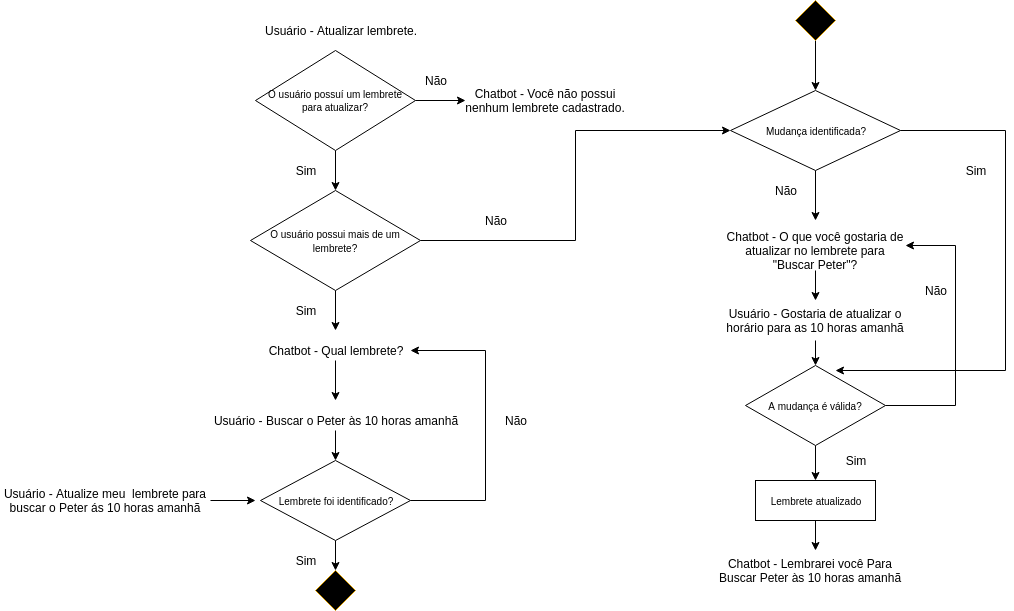
\includegraphics[width=0.9\linewidth]{src/imagens/Chatbot.png}
\caption{\textit{Chatbot flowchart}} Fonte:~\cite{Samer}
\label{cap:01:fig:fluxograma}
\end{figure}

Outra característica importante nesse tipo de \textit{chatbots}, é que eles não precisam necessariamente compreender a linguagem humana para executarem suas tarefas~\cite{Juliano}.

\subsection{\textit{Chatbots} de domínio amplo}\label{cap:02:sec:01:sub:02:bot-dominio}

Já os \textit{chatbots} de domínio amplo utilizam de recursos mais avançados de Inteligência Artificial (\abrv[IA - Inteligência Artificial]{IA}), são capazes de compreender o que o usuário solicita e podem relacionar-se a qualquer área de domínio de conhecimento~\cite{Juliano}. 
Na maior parte do tempo, o atendimento realizado por esse tipo de \textit{chatbots}, procura simular a conversação em linguagem humana.
Em outras palavras, um dos objetivos principais é responder perguntas de forma que os usuários tenham a impressão de estarem conversando com outra pessoa e não com um programa de computador.
Para isso, são utilizadas técnicas de Aprendizagem de Máquina (\textit{Machine Learning}) ou de Processamento de Linguagem Natural (\textit{Natural Language Processing})~\cite{Falaki}. 
Assim, o \textit{chatbot} é treinado com base nas interações dos usuários e consegue aprender com elas, se tornando mais inteligente e preciso ao decorrer deste processo.

As Assistentes Virtuais Inteligentes (\abrv[AVIs - Assistentes Virtuais Inteligentes]{AVIs}) são um dos exemplos de \textit{chatbots} desse tipo. 
As AVIs são uma das principais tendências de soluções para otimizar o relacionamento entre empresas e consumidores~\cite{DDS}. 
Por meio de mecanismos de Inteligência Artificial, elas aprendem a partir das interações com o consumidor e, com isso, melhoram o seu repertório. 
Assim, são capazes de entender as necessidades do cliente e auxiliá-los da devida maneira na resolução de seus problemas.

\section{Inteligência artificial para \textit{chatbots}}\label{cap:02:sec:02:ia}

\subsection{Aprendizado de máquina}\label{cap:02:sec:02:sub:machine-learning}

De maneira simplificada, Aprendizagem de máquina é a prática de usar algoritmos para coletar dados, aprender com eles, e então fazer uma determinação ou predição sobre alguma atividade específica~\cite{SimpleML}. Assim ao invés de implementar as rotinas de software propriamente ditas, com um conjunto específico de instruções para completar uma tarefa em particular, a máquina é “treinada” usando uma quantidade grande de dados e algoritmos que dão e ela a habilidade de aprender como executar a tarefa. De maneira mais técnica, é um método de análise de dados que automatiza a construção de modelos analíticos~\cite{SASML}. Se baseia na ideia de que sistemas podem aprender com dados, identificar padrões e tomar decisões com o mínimo de intervenção humana.

Existem vários serviços que fornecem e facilitam o uso de tecnologias de aprendizagem de máquina, um deles, por exemplo, é a Amazon Machine Learning.
O Amazon Machine Learning oferece ferramentas e assistentes de visualização que orientam o desenvolvedor durante o processo de criação de modelos de aprendizado de máquina, sem necessidade de aprender tecnologias e algoritmos complexos para o desenvolvimento de tal. 


\subsection{Processamento de Linguagem Natural}\label{cap:02:sec:02:sub:pln}

O Processamento de Linguagem Natural (\abrv[PLN - Processamento de Linguagem Natural]{PLN}) é a subárea da IA que estuda a capacidade e as limitações de uma máquina em entender a linguagem dos seres humanos~\cite{PLN1}.
Alguns dos objetivo do PLN é fornecer aos computadores a capacidade de  reconhecer o contexto, fazer análise sintática, semântica, léxica e morfológica, criar resumos, extrair informação, interpretar os sentidos, analisar sentimentos e até aprender conceitos com os textos processados~\cite{PLN1}.

Um dos métodos utilizados do PLN para o desenvolvimento de \textit{chatbots} é transformar uma sentença textual (dado) em informação (intenção e entidades)~\cite{Anatomy}. Em outras palavras, as intenções expressam funcionalidades, entidades expressam parâmetros para a execução de uma funcionalidade. Essas entidades precisam ser cadastradas, de forma a servir à base de conhecimento do PLN. Depois criamos as intenções, onde determinamos frases e sentenças que usarão essas entidades para expressar essas intenções. Assim, de modo simplório, o PLN passa a conseguir interpretar textos completos, textos simples e até mesmo incompletos.

Atualmente, existem vários serviços que dão suporte para a criação de PLN, um desses exemplos é o Wit.ia. Wit.ai é uma plataforma de desenvolvimento de PLN gratuita que transforma a linguagem natural (fala ou escrita) em dados estruturados. Um dos principais motivos para o uso do Wit.ai é por sua simplicidade no processo de criação de aplicativos e dispositivos com os quais as pessoas podem conversar, nesse contexto, na criação de \textit{chatbots}. Com isso, se abstrai a necessidade de aprender todo o processo de desenvolvimento de algoritmos de PLN.


\section{\textit{Chatbots} em plataformas de mensagens instantâneas}\label{cap:02:sec:03:sub:chatbotsmessenger}

Um mensageiro instantâneo consiste em um software que permite que diferentes usuários troquem mensagens, geralmente por escrito, em tempo real. 
Esses mensageiros instantâneos podem possuir alguns recursos adicionais como o envio de arquivos, conversas de áudio, conversas coletivas e até video conferências.
O termo mensageiro instantâneo, no entanto, encontra-se em desuso, sendo agora chamado com mais frequência por plataformas de mensagens instantâneas, ou simplesmente por \textit{messengers}. Podemos citar alguns \textit{messengers} como exemplo, tais como o Whatsapp, Telegram, WeChat, Slack, Facebook Messenger, entre outros.

No que se diz respeito à criação de \textit{chatbots}, alguns desses \textit{messengers} oferecem ferramentas e suporte, sob licenças especificas, para o desenvolvimento em sua plataforma, por meio de \textit{Application Programming Interfaces} (APIs).
Dentre os \textit{messengers}, um dos mais famosos por possuírem tais funcionalidades, é o Telegram.
O Telegram foi lançado em 2015 e possuí cerca de 100 milhões de usuários ativos mensais~\cite{IMaster}, 
É válido ressaltar também, os seus recursos avançados em questão de segurança e criptografia.
O Telegram oferece suporte para desenvolvimento de \textit{chatbots} desde 2015, por meio de sua API baseada no protocolo \abrv[HTTP - Hypertext Transfer Protocol]{HTTP} (Hypertext Transfer Protocol).


\section{Projetando \textit{chatbots}}\label{cap:02:sec:05:projeto}

Como sistemas computacionais são construídos para terem utilidade no mundo real, modelar o domínio de aplicação é uma atividade de suma importância.
A partir dessa atividade, pode se compreender a necessidade do sistema a ser construído e também definir os requisitos que tornam o sistema útil~\cite{ReqJair}. 
Pelo fato do \textit{chatbot} também se tratar de um produto digital, algumas práticas e estudos também devem ser realizados em seu processo de criação. Algumas dessas pŕaticas envolvem a análise e especificação dos requisitos e a elaboração dos diálogos que farão parte do repertório de um \textit{chatbot}.

\subsection{Análise e especificação dos requisitos}

De acordo com \alusao{ReqJair} a análise e especificação de requisitos de software envolve as atividades de determinar os objetivos de um software e as restrições associadas a ele.
\alusao{ReqJair} diz que a análise é o processo de observação e levantamento dos elementos do domínio no qual o sistema será introduzido. Deve-se identificar  as pessoas, atividades, informações do domínio para que se possa decidir o que deverá ser informatizado ou não.
Já a especificação é a descrição sistemática e abstrata do que o software deve fazer, a partir daquilo que foi analisado.

\subsubsection{Classificação de requisitos}\label{cap:02:sec:05:projeto:classificacao-requisitos}

\alusao{Sommerville} estabelece que os requisitos de um sistema são as descrições do que o sistema deve fazer, os serviços que oferece e as restrições a seu funcionamento.
Esses requisitos refletem as necessidades dos clientes para um sistema que serve a uma finalidade determinada, como controlar um dispositivo, efetuar um pedido ou encontrar informações.
É válido ressaltar que os requisitos de software são frequentemente classificados como requisitos funcionais e requisitos não funcionais.

Os requisitos funcionais de um sistema descrevem o que ele deve fazer.
Eles dependem do tipo de software a ser desenvolvido, de quem são seus possíveis usuários e da abordagem geral adotada pela organização ao escrever os requisitos~\cite{Sommerville}.
Quando expressos como requisitos de usuário, os requisitos funcionais são normalmente descritos de forma abstrata, para serem compreendidos pelos usuários do sistema.\label{texto:requisito_funcional}

Já os requisitos não funcionais, como o nome sugere, são requisitos que não estão diretamente relacionados com os serviços específicos oferecidos pelo sistema a seus usuários~\cite{Sommerville}.
Eles podem estar relacionados às propriedades emergentes do sistema, como confiabilidade, tempo de resposta, integridade, disponibilidade, ocupação de área entre outros.\label{texto:requisito_nao_funcional}

\subsection{Especificando requisitos utilizando casos de uso}

De acordo com \alusao{ReqJair} um caso de uso especifica o comportamento do sistema a ser desenvolvido sem, no entanto, especificar como este comportamento será implementado.
Os comportamentos descrevem as funções da aplicação que caracterizam a funcionalidade do sistema.
Um caso de uso representa o que o sistema faz e não como o sistema faz, proporcionando uma visão externa e não interna do sistema. Cada caso de uso define um requisito funcional do sistema~\cite{ReqJair}.

O caso de uso descreve um conjunto de sequências de ações que o sistema desempenha para produzir um resultado esperado pelo usuário.
Cada sequência representa a interação de entidades externas e o sistema~\cite{ReqJair}.
Estas entidades são chamadas de atores e que podem ser usuários ou outros sistemas.
No caso de usuários, um ator representa na verdade uma função de usuários. Para isso, normalmente se utiliza da notação \abrv[UML - Unified Modeling Language]{UML} (\textit{Unified Modeling Language}) como linguagem de especificação para representar os casos de uso. Na Figura~\ref{cap:02:fig:caso-de-uso-exemplo}, segue um exemplo de especificação de casos de uso utilizando a notação UML de um sistema de vendas.\label{texto:especificando-com-casos-de-uso}

\begin{figure}[htb!]
\centering
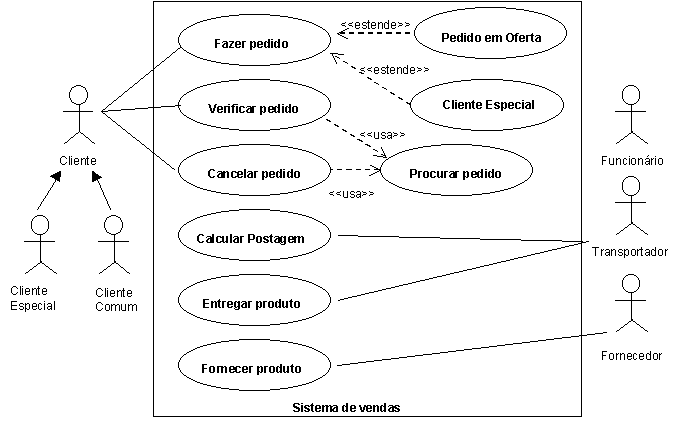
\includegraphics[width=0.7\linewidth]{src/imagens/casosd2.png}
\caption{Caso de uso - Sistema de Vendas} Fonte:~\cite{ReqJair2}
\label{cap:02:fig:caso-de-uso-exemplo}
\end{figure}

\subsection{Elaboração dos diálogos de um \textit{chatbot} a partir de cenários}\label{texto:elaborando-dialogos}

Para a elaboração dos diálogos que irão fazer parte do repertório de um \textit{chatbot}, uma técnica utilizada para a sua modelagem e especificação se dá pelo uso dos cenários.
\alusao{ReqJair} diz que cenários consistem de uma coleção de narrativas de situações no domínio que favorecem o levantamento de informações, a identificação de problemas e a antecipação das soluções.
Cenários são uma maneira de representar, no contexto de \textit{chatbots}, os diálogos e interações e as possibilidades que podem surgir a partir destes. Abaixo, um exemplo de cenário que simula o diálogo entre uma atendente e um cliente que deseja consultar seu histórico de compras:


\begin{itemize}
    \item \textbf{Suposição inicial:}
    
    O cliente informa que deseja consultar o seu histórico de compras; a atendente pergunta suas informações pessoais (nome e CPF); o cliente informa seus dados; a atendente faz uma consulta com base nos dados adquiridos; a atendente exibe o histórico de compras do cliente.
    
    \begin{enumerate}
        \item \textbf{Cliente}: Gostaria de consultar meu histórico de compras, por favor.
        \item \textbf{Atendente}: O senhor poderia me informar o seu nome completo e os três últimos dígitos do seu CPF?
        \item \textbf{Cliente}: Claro. Meu nome é Custódio de Almeida, e os três últimos dígitos do meu CPF são 186.
        \item \textbf{Atendente}: Um instante, por favor.
        \item \textbf{Atendente}: O histórico do senhor é o seguinte: \\
        Dia: 20/02/2017 - 1 Tênis branco da marca X, 2 camisetas rosas da marca Y.\\
        Dia: 25/02/2017 - 2 shorts amarelos da marca Z.
        \ldots
    \end{enumerate}
    
    \item \textbf{O que pode dar errado:}
    
    As informações fornecidas pelo usuário não conferem com as cadastradas no banco de dados. A atendente informa o usuário que os dados informados não são válidos e pede para que ele tente novamente.
    
    \begin{enumerate}
        \item \textbf{Atendente}: Me desculpe, mas parece que os dados informados não conferem. Você poderia tentar novamente?
        \item \textbf{Cliente}: Certo. Tente os seguintes dados dessa vez \ldots
    \end{enumerate}
    
    O usuário nunca efetuou uma compra no estabelecimento. A atendente informa que o usuário não tem nenhuma compra na loja e informa as promoções disponíveis.
    
    \begin{enumerate}
        \item \textbf{Atendente}: Me desculpe, mas parece que o senhor não possui nenhuma compra em nossa loja.
        \item \textbf{Cliente}: Tudo bem, então.
        \item \textbf{Atendente}: Caso seja do seu interesse, nós estamos com uma promoção de 30\% de desconto na compra de qualquer camiseta da marca X. Você gostaria de dar uma olhada? \ldots
    \end{enumerate}
    
    \item \textbf{Estado do sistema na conclusão:}
    
    Após exibir o histórico do cliente, a atendente irá perguntar se o ele deseja mais alguma coisa.
    
    \begin{enumerate}
        \item \textbf{Atendente}: Esse é todo o seu histórico de compras em nossa loja. Existe mais alguma coisa em que eu possa lhe ajudar?
        \ldots
    \end{enumerate}
    
    
\end{itemize}


\section{Desenvolvimento de \textit{chatbots}}\label{chatbot:dev}

No desenvolvimento de \textit{chatbots}, pode-se dizer que existem duas maneiras para a sua criação: utilizando ferramentas de plataformas de \textit{chatbots} ou não. Para melhor explicar a vantagens e desvantagens de cada modo, nas subseções abaixo, estes serão detalhados.

\subsection{Utilizando plataformas de \textit{chatbots}}\label{chatbot:dev:plat}

A plataformas de \textit{chatbots} são sistemas que oferecem serviços para facilitar a criação de \textit{chatbots} e sua integração com os  \textit{messengers}.
Basicamente, essas plataformas abstraem a necessidade de programar rotinas de códigos complexas, já oferecem recursos ou serviços de IA embutidos e também a tradução da aplicação, aonde o \textit{chatbot} poderá ser exportado e integrado para os mais diversos \textit{messengers}.
O intuito dessas plataformas, é elevar a produtividade dos desenvolvedores responsáveis pela criação do \textit{chatbot}.
Assim, ao facilitar o processo de criação, abstraindo várias etapas complexas e trabalhosas, eles serão capazes de desenvolverem o \textit{chatbot} em menos tempo.
Como exemplo dessas plataformas de \textit{chatbots}, podemos citar a Microsoft Bot Plataform, ChatScript, Pandorabots, Facebook Bots for Messenger, BLIP, entre outros.

Porém, para que possam se utilizar dos recursos mais avançados dessas plataformas, as empresas ou desenvolvedores contratantes devem efetuar os pagamentos, que podem variar de acordo com o tipo de serviço solicitado, podendo estes serviços serem mais caros de acordo com o número de usuários simultâneos que o \textit{chatbot} poderá atender, até, em questões de utilização de recursos mais sofisticados e personalizados para agilizar no desenvolvimento dos \textit{chatbots}. 


\subsection{Não utilizando plataformas de \textit{chatbots}}\label{chatbot:dev:nplat}

Caso o desenvolvedor opte pela não utilização dessas plataformas de \textit{chatbots}, ele poderá customizar a sua aplicação utilizando as tecnologias, ferramentas e serviços que lhe bem convir.
Por exemplo, ele poderá escolher desde de uma linguagem de programação específica até qual serviço de IA (caso seja um \textit{chatbot} de domínio amplo) que ele irá utilizar no projeto.
Como dito na seção \ref{cap:02:sec:03:sub:chatbotsmessenger}, muitos \textit{messengers} oferecem suporte e serviços, por meio de suas APIs, que facilitam o processo de desenvolvimento e integração do \textit{chatbot} em sua plataforma.
Assim, o desenvolvedor poderá avaliar dentre os serviços oferecidos por esses \textit{messengers} e escolher qual lhe oferece mais benefícios.

É válido ressaltar a existência de bibliotecas que facilitam ainda mais o de desenvolvimento de \textit{chatbots}.
Essas, por sua vez, abstraem algumas etapas no processo de criação e integração dos \textit{chatbots} com os \textit{messengers}.
Podemos resumi-las em uma implementação real das regras de uma API de um \textit{messenger}, no contexto de \textit{chatbots}, elas oferecem uma interface mais simplificada para o seu desenvolvimento, utilizando alguma linguagem de programação específica, aonde se abstrai, por exemplo, a necessidade de programar rotinas que possibilitem a comunicação do \textit{chatbot}, via algum protocolo pré-determinado, com a API do \textit{messenger}.
